\section{Command-Processor Model and Formulation}
\label{sec:model}

% VALUE: we first establish how the CP turns instruction streams into overlap, on the existing prefill's own operators, then state the scheduling problem these semantics define
In this section, we present how the CP turns instruction streams into overlap, and the scheduling problem that these semantics define.
We characterize the semantics on the existing prefill's own operators, pairing one attention operator on columns 0 and 7 with one GEMM operator on columns 1--6.
Every composed command in this section produces outputs bit-identical to those of the operators run alone.

\subsection{Concurrency Semantics}
\label{subsec:semantics}

\begin{figure}[t]
    \centering
    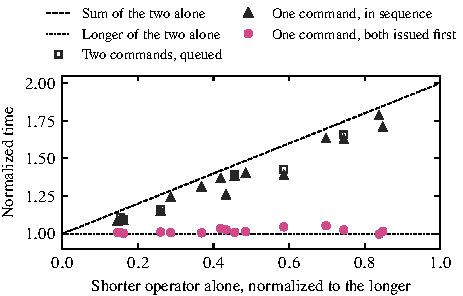
\includegraphics[width=\linewidth]{fig/pairs.pdf}
    % VALUE: queued commands take the sum of the two operators, one command that issues both before waiting takes the longer one
    \caption{Median time of one attention and one GEMM operator on disjoint column groups, normalized to the longer operator alone, over 20 runs per pair. Holding both streams in one command saves one dispatch floor against the sum.}
    \label{fig:pairs}
\end{figure}

\textbf{Queued Commands.}
% VALUE: the runtime gives no overlap across commands, and placing two operators in one command is itself neutral, so overlap must come from within a command
Two commands queued on one hardware context, with no wait between them, take as long as one command that holds both streams in sequence, within 3\% on every pair (Figure~\ref{fig:pairs}).
Holding both streams in sequence in one command takes the sum of the two operators' times minus one dispatch floor, within 2\%, so placing two operators in one command is itself neutral.
The hardware context therefore executes commands strictly one after another, and any overlap between operators must come from within a single command.
% SOURCE: queued / in-sequence = 1.007-1.029 on 7 pairs (amd-npu 17f7ec3 prefill-overlap/ovl4/, lab-prefill-overlap (5)b); in-sequence / (A + G - F) = 0.996-1.021 over 17 pair runs (ovl/, ovl2/ at 8f13e05 and ovl4/; report.txt H1 column).

\textbf{Concurrent Issue.}
% VALUE: one command that issues both groups' work before it waits on either runs them concurrently at nearly the longer one's time; the small cost appears when both read DRAM near the cap
When one command issues all of the GEMM's work, then the attention operator's stream, and only then the GEMM's synchronizations, the two operators run concurrently.
Such a command takes 1.00--1.06 times the longer operator's time on 9 pairs that cover three GEMM shapes and attention over chunks 0 to 15 (Figure~\ref{fig:pairs}).
On six further pairs with other shapes and chunks, the overlap hides 90--96\% of the shorter operator's work, after excluding the dispatch floor that the merge already saves.
The overlap costs most when the pair's combined DRAM read rate approaches the read cap, at about 95\% of the cap measured in the same batch.
The serial execution of the existing prefill is therefore a property of how its commands are composed, not of the array or its configuration.
% SOURCE: interleaved / max(A, G) = 0.998-1.058 over 10 pair runs = 9 pairs (c8 + lm measured twice, 1.054 and 1.058; the figure keeps each pair's first measurement); GEMM shapes up, LM head chunk, down; attention chunks 0, 4, 8, 12, 15 (lab-prefill-overlap (3)).
% SOURCE: hidden fraction of the shorter operator's work, (in-sequence - interleaved) / (min(A, G) - F) = 0.90-0.96 on 2+qkv, 6+o, 11+gate, 14+qkv, 6+gate, 11+o (lab-prefill-overlap (5)a).
% SOURCE: DRAM rate during the interleaved command 52.2 GB/s against a same-batch 8x2 cap of 53.9-55.3 GB/s for c8 + lm, the largest overlap cost (1.054-1.058) (lab-prefill-overlap (3)).

\textbf{Synchronization Order.}
% VALUE: because the CP is in order, a wait on one group delays the issue of every other group's work; the existing attention stream loses a third of its busy time this way, inside a single operator
Since the CP executes in order, a synchronization on one group delays every later issue, including the issue of another group's work.
The existing attention operator shows the cost within a single operator: its stream issues column~7's inputs only after two synchronizations on column~0's key and value transfers, which complete when column~0 is about half done.
Alternating the two columns' segments, so that both columns start before the CP waits on either, reduces attention's device-busy time to $0.67\times$ that of the existing order at every chunk measured, with bit-identical outputs.
Each column's half alone takes the same time within 1\%, so the difference comes from the CP's instruction order rather than from an imbalance of work.
The CP's instruction order, and not only the assignment of operators to commands, is therefore a scheduling decision.
% SOURCE: decoded from the shipped a_32_4_0_0 stream, mid-stream synchronizations at ops 70, 75 (column 0) and 92, 97 (column 7); column 7's issue (ops 81-91) follows column 0's two mid-stream synchronizations (lab-prefill-overlap (4)).
% SOURCE: (alternated - F) / (existing - F) = 0.666-0.668 on 7 pairs, chunks 2-14 at 2,048 tokens; column 7 alone / column 0 alone = 0.994-1.010 (amd-npu 17f7ec3 ovl4/, lab-prefill-overlap (5)c).

\subsection{Problem Formulation}
\label{subsec:formulation}

\textbf{Resources.}
% VALUE: three kinds of resources: column groups (one operator at a time, data-driven), the CP (one in-order server that issues and blocks), and the host (work between commands)
The array offers a set $\mathcal{G}$ of disjoint column groups, each running one operator at a time and sharing only DRAM bandwidth with the others.
The CP is a single in-order server that executes issue instructions, each at a small cost, and blocks at each synchronization until the transfer it names completes.
The host CPU runs the work between operators that the array does not perform, such as normalizations, and it submits and collects commands.

\textbf{Operators.}
% VALUE: each operator is defined by its group, its device time, its host work, and its instruction stream split into segments; dependencies pass through DRAM and need a synchronization
Each operator $o \in \mathcal{O}$ runs on group $g(o)$ for a device-busy time $p_o$, and may need host work of duration $h_o$ after it completes.
Its instruction stream is a sequence of \emph{segments} $s_{o,1}, \dots, s_{o,n_o}$, where each segment consists of synchronizations followed by the issue instructions they gate, and the first segment has no synchronizations.
A dependency graph $E \subseteq \mathcal{O} \times \mathcal{O}$ orders the operators.
Since operators hand data over through DRAM, with no lock on the device between them, a consumer's first issue must follow the producer's final synchronization.
When host work lies between producer and consumer, the consumer must also wait for that host work, and the two cannot share a command.

\textbf{Decisions.}
% VALUE: the essential decisions are the spatial assignment and the CP's instruction order; the command partition and the queue depth manage host boundaries and are reported apart
A schedule makes two essential decisions.
The first is the spatial assignment $g(\cdot)$ of operators to column groups, which determines what can run concurrently.
The second is the CP's instruction order, namely a partition of $\mathcal{O}$ into a sequence of commands $C_1, \dots, C_K$ and, for each command, an interleaving $\sigma_k$ of its operators' segments that keeps each operator's segments in their own order.
Two further decisions manage the boundaries with the host: how many commands the host keeps in flight, and how operators that do not overlap are packed into commands.
Both would disappear if the host work moved onto the array, so we report their effect separately from that of the essential decisions.

\textbf{Timing.}
% VALUE: the semantics of Section 3.A as rules: commands in sequence with a boundary cost; within a command, a segment's work starts once issued and its predecessor has finished; a synchronization completes when its work has
A command starts on the device after its predecessor completes, plus a \emph{boundary cost} $\epsilon$ when it was already queued, or the dispatch floor $F$ when it arrives at an idle device.
Within a command, the CP walks $\sigma_k$ in order.
The work of segment $s_{o,j}$ starts on $g(o)$ once the CP has issued it and the work of $s_{o,j-1}$ has finished, and a synchronization completes once the CP reaches it and the work it names has finished.
Operators that run at the same time on different groups take longer than alone by an overlap cost that grows with their combined DRAM traffic.

\textbf{Objective.}
% VALUE: minimize the makespan, which for prefill is TTFT less a fixed head and tail
The objective is the makespan, i.e., the completion time of the last command, which for prefill is the TTFT less a fixed head and tail of work outside the layers.

\subsection{Lower Bound}
\label{subsec:bound}

% VALUE: each of the three resources bounds the makespan, so their maximum bounds the gap of any schedule on a given assignment
Each resource bounds the makespan from below:
\begin{equation}
\label{eq:lb}
T \;\ge\; \max\Bigl(\max_{g \in \mathcal{G}} \sum_{o:\,g(o)=g} p_o,\;\; L_E,\;\; \sum_{k} c_k\Bigr),
\end{equation}
where $L_E$ is the longest path through $E$ weighted by $p_o$ plus, on host-crossing edges, $h_o$, and $c_k$ is the CP's own work in command $k$.
The first term is the busiest group's work, which no schedule on a fixed assignment can beat.
The bound therefore measures how far a schedule lies from what a given spatial assignment allows.
% DECISION: the bound's value for the studied instances, from the measured per-operator times, is stated with the evaluation's gap.
% DECISION: no NP-hardness claim until a reduction is written; with negligible issue cost and one layer's fixed per-chunk pattern the problem has the structure of a two-machine chain-reentrant shop (wang1997reentrant), and with non-negligible issue cost the CP acts as a shared server (glass2000dedicated, hall2000common) (vault ch3-formulation, Relation to classical scheduling).
